Ta có với OPAMP trên mắc theo kiểu Vi sai nên ta có phương trình như sau:
\begin{center}
	\finalresult{V_{o} = \dfrac{R_{2}}{R_{1}} \left(V_{1} - V_{2}\right) = 3\left(V_{1} - V_{2}\right)}
\end{center}

\begin{figure}[H]
	\centering
	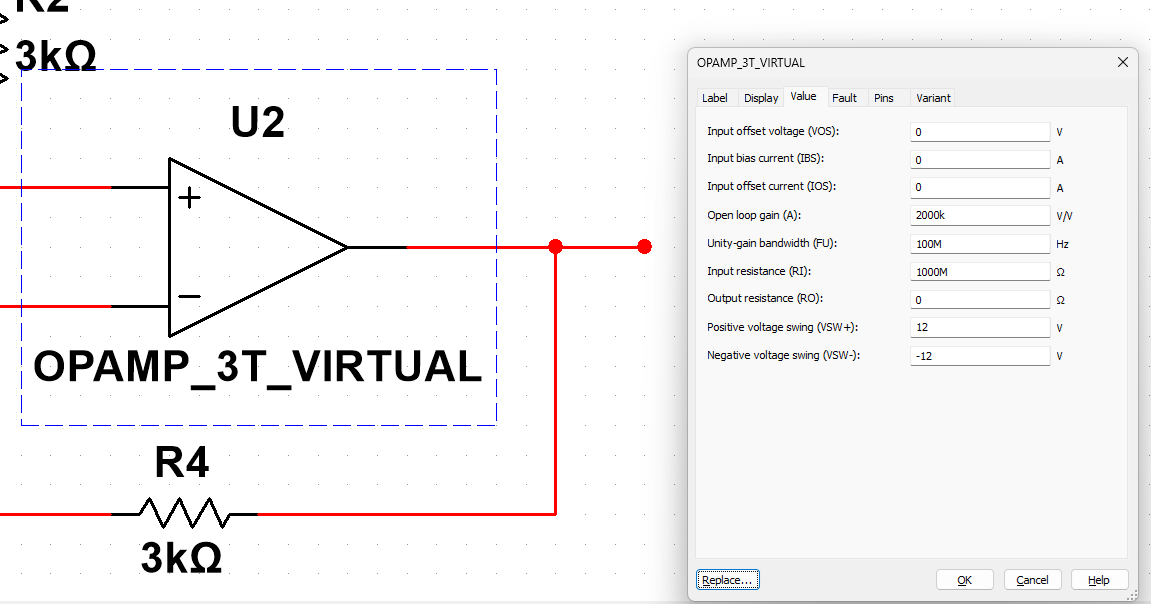
\includegraphics[width=.4\linewidth]{./my-chapters/my-images/Question5/a/a_setup_opamp_ideal.png}
	\caption{Setup giá trị cho OPAMP lý tưởng.}
\end{figure}

Với 1 OPAMP lý tưởng thì các giá trị như sau:

\begin{itemize}[label=-]
	\item Input offset voltage: $V_{OS} = 0\,\textsf{V}$
	\item Input bias current: $I_{BS} = 0\,\textsf{V}$
	\item Input offset current: $I_{OS} = 0 \,\textsf{V}$
	\item Open loop gain: $A = \infty \,\textsf{V/V}$
	\item Unity-gain bandwidth: $FU = \infty\,\textsf{Hz}$
	\item Input resistance: $R_{I} = \infty\,\Omega$
	\item Ouput resistance: $R_{O} = 0\,\Omega$
\end{itemize}

\begin{figure}[H]
	\centering
	
\includegraphics[width=.8\linewidth]{./my-chapters/my-images/Question5/a/a_machmophong.png}
	\caption{Mạch mô phỏng với OPAMP lý tưởng.}
\end{figure}

\begin{figure}[H]
	\centering
	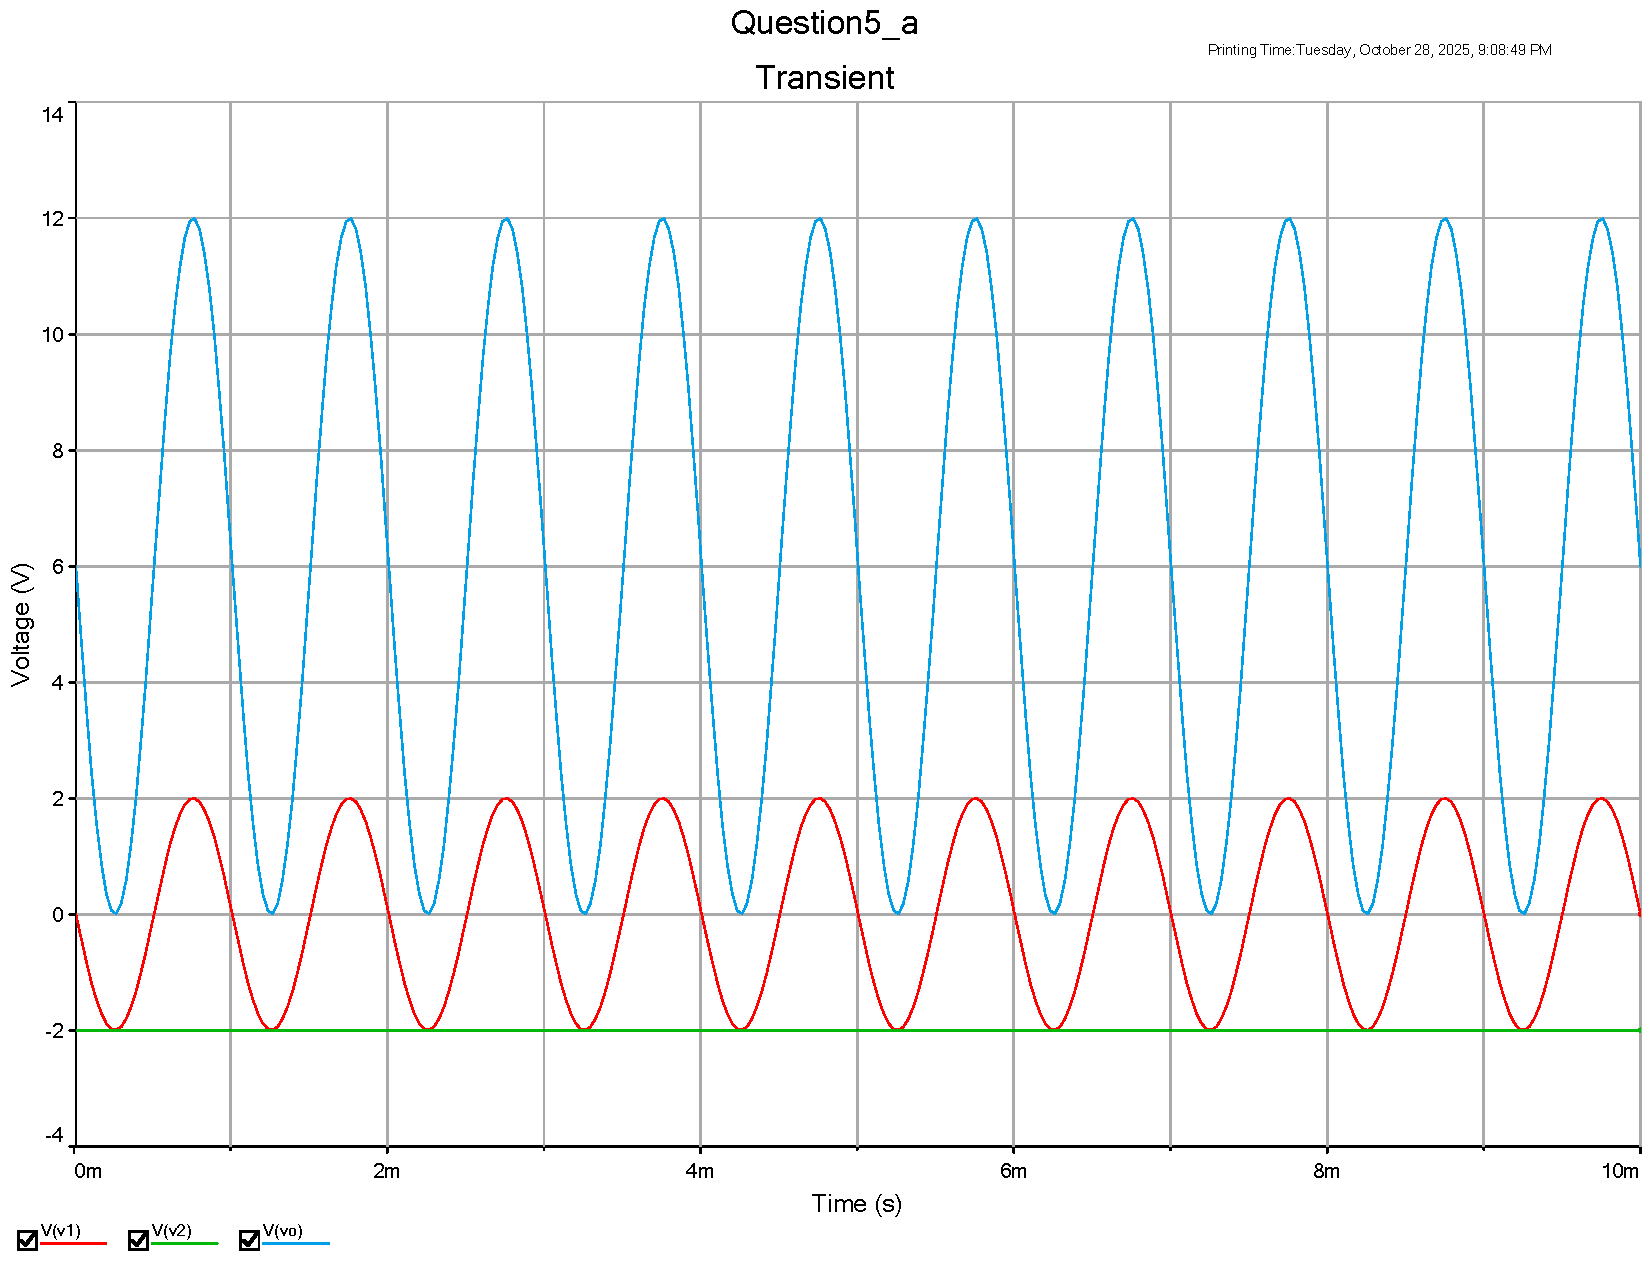
\includegraphics[width=.8\linewidth]{./my-chapters/my-diagrams/Question5/a_dangsongngora.pdf}
	\caption{Dạng sóng ngõ ra nếu OPAMP là lý tưởng.}
\end{figure}

\begin{itemize}[label=-]
	\item Với $V_{1} = 0\text{, }V_{2} = -2 \Rightarrow V_{o} = 3\left( 0 - -2\right) = 6\,\textsf{V}$
	\item Với $V_{1} = -2\text{, }V_{2} = -2 \Rightarrow V_{o} = 3\left( -2 - -2\right) = 0\,\textsf{V}$
	\item Với $V_{1} = 2\text{, }V_{2} = -2 \Rightarrow V_{o} = 3\left( 2 - -2\right) = 12\,\textsf{V}$
\end{itemize}